\chapter{既存手法}\label{cha:Function}

本章では、既存手法について説明する。
既存手法は、自然言語仕様書を入力として、型定義と定数定義を記述したVDM++仕様書を出力する。

既存手法の構造を、図\ref{fig:exis_structure}に示す。既存手法は、以下の4つの処理部で構成する。

\begin{figure}[tp]
    \begin{center}
        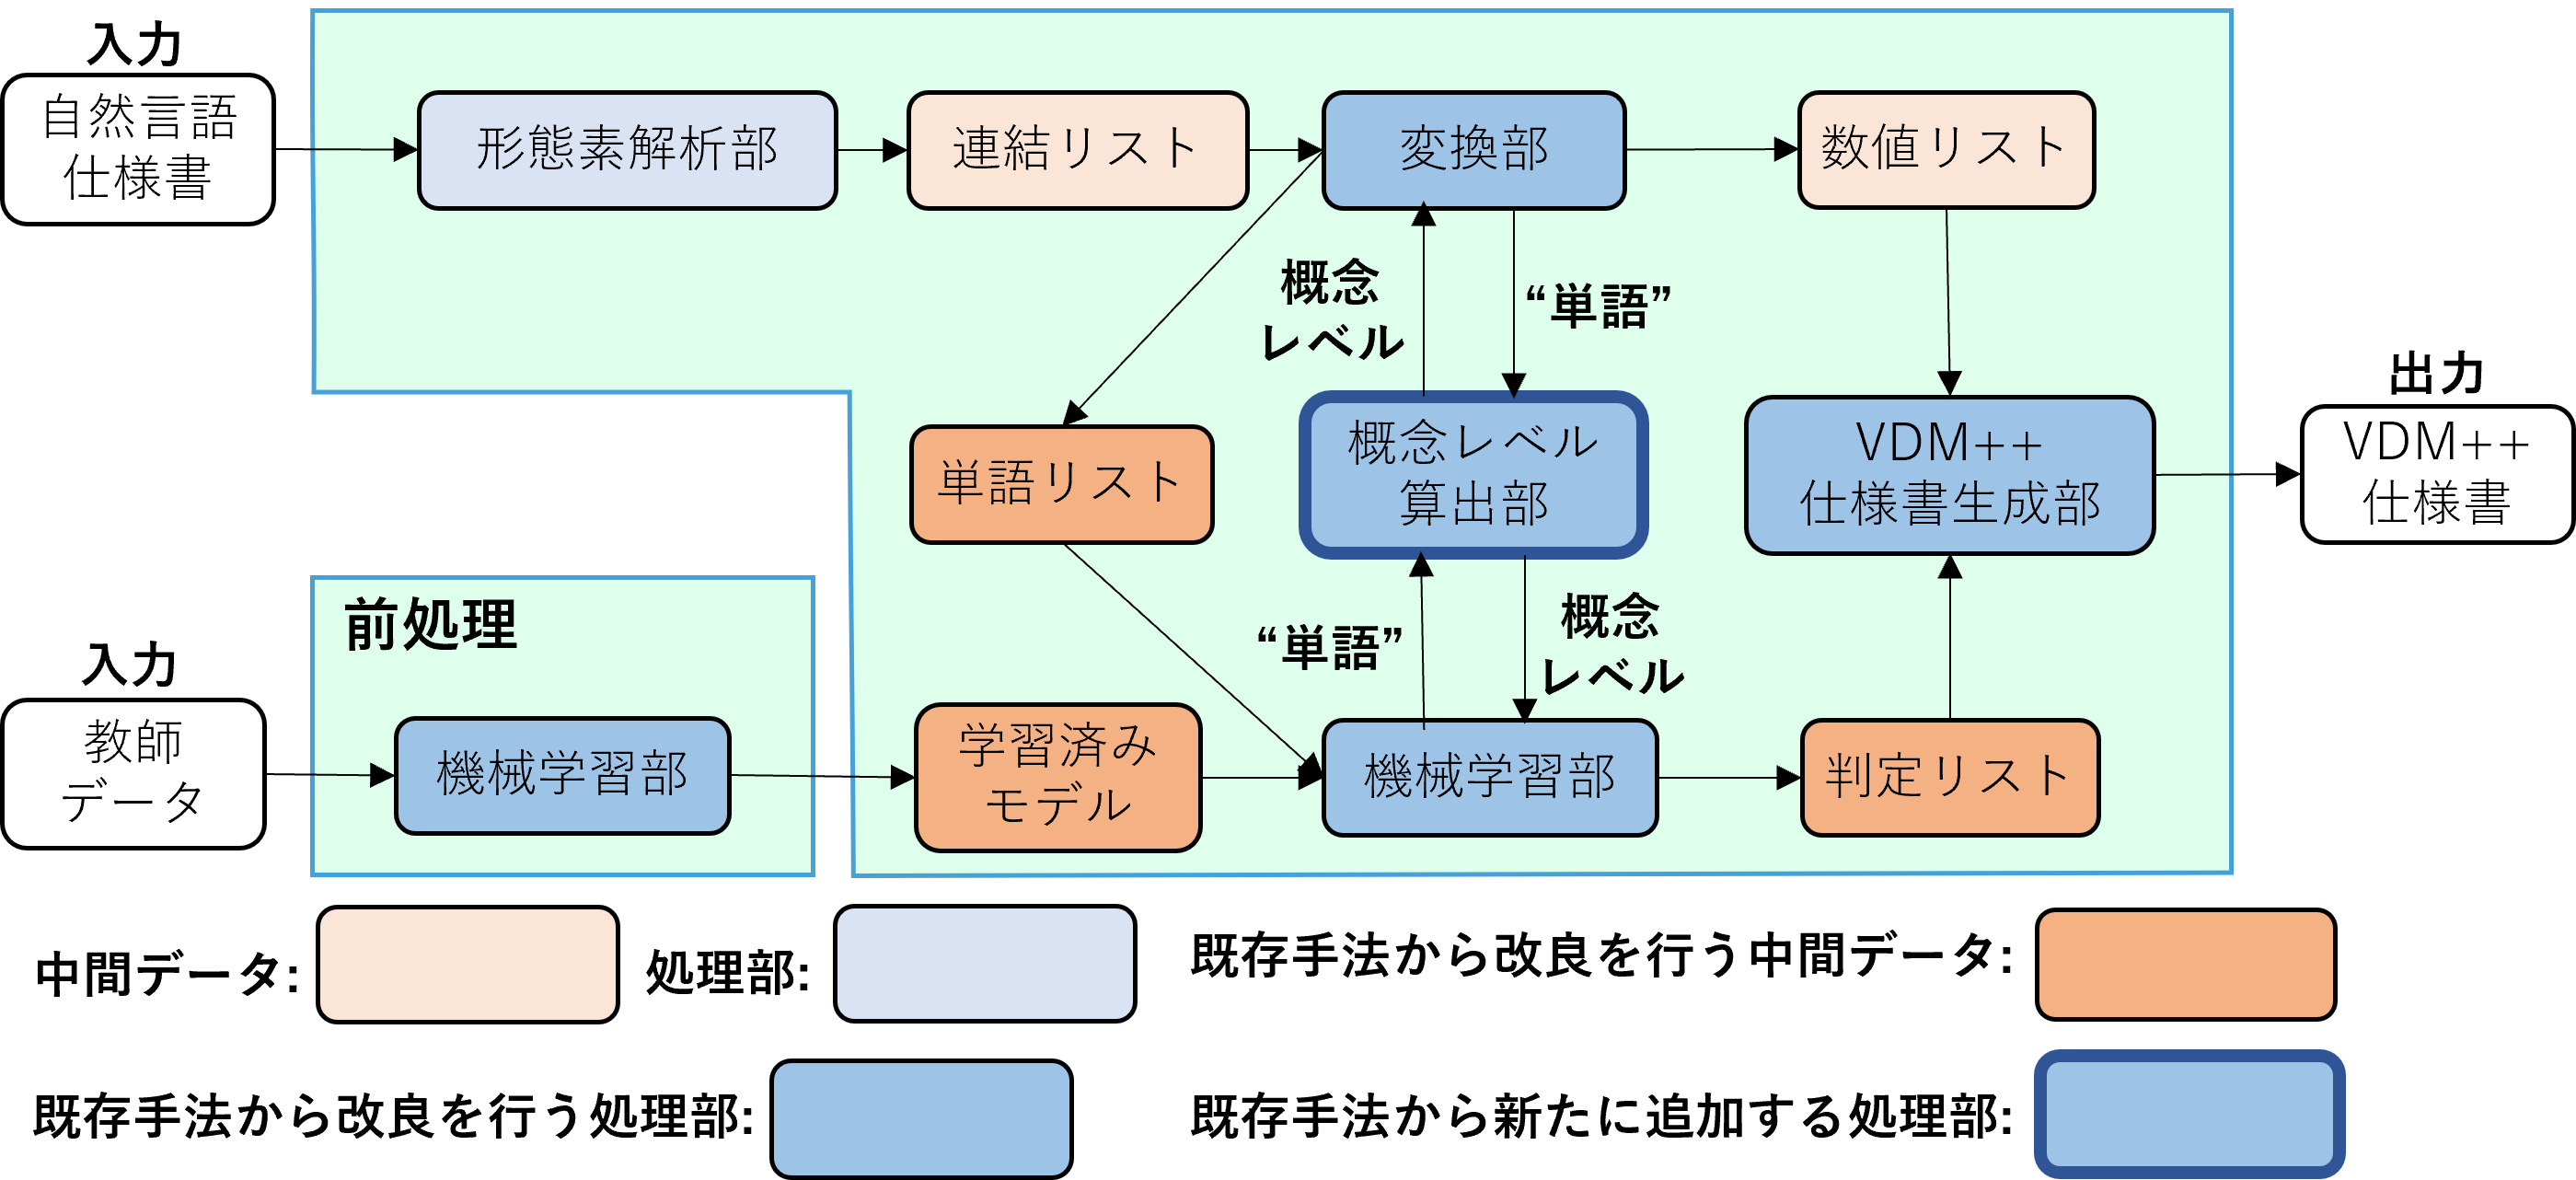
\includegraphics[width=1.0\columnwidth]{image/vgml_structure.png}
        \caption{既存手法の構造}
        \label{fig:exis_structure}
    \end{center}
\end{figure}

\begin{itemize}
    \item 形態素解析部
    \item 変換部
    \item 機械学習部
    \item VDM++仕様書生成部
\end{itemize}

以降、4つの処理部について詳細を説明する。

\section{形態素解析部}
既存手法における形態素解析部は、wordまたはpdfで記述された自然言語仕様書を入力として、連結リストを出力する。
既存手法が入力とする自然言語仕様書の例を図\ref{fig:exis_spec_example}に、既存手法における形態素解析部の構造を、図\ref{fig:exis_mor_structure}に示す。
既存手法における形態素解析部の処理の流れを、以下に示す。

\begin{enumerate}
    \item テキスト抽出処理において、自然言語仕様書を入力とし、自然言語仕様書内のテキストを抽出する。さらに、抽出したテキストを格納したテキストリストを生成する。図\ref{fig:exis_spec_example}に示す仕様書を入力として、既存手法のテキスト抽出処理が生成するテキストリストを、図\ref{fig:exis_text_list}に示す。
    \label{text_list}
    \item 分かち書き処理において、\ref{text_list}で生成したテキストリストを入力とし、テキストリスト内のテキストを文ごとに分ける。さらに、文を\ref{}節で述べたMecabを用いて分かち書きし、分かち書きした文を格納した分かち書きリストを生成する。図\ref{fig:text_list}に示すテキストリストを入力として、既存手法の分かち書き処理が生成する分かち書きリストを、図\ref{fig:exis_wakati_list}に示す。
    \label{wakati_list}
    \item 単語連結処理において、\ref{wakati_list}で生成した分かち書きリストを入力とし、分かち書きリスト内の助詞、助動詞、接続詞、副詞の品詞である単語を除く。さらに、分かち書きリスト内の文の連続する2つ以上の名詞と動詞を連結する。最後に、名詞と動詞を連結した文を格納した連結リストを生成する。図\ref{fig:wakati_list}に示す分かち書きリストを入力として、既存手法の単語連結処理が生成する連結リストを、図\ref{fig:exis_connect_list}に示す。
\end{enumerate}

\begin{figure}[tp]
    \begin{center}
        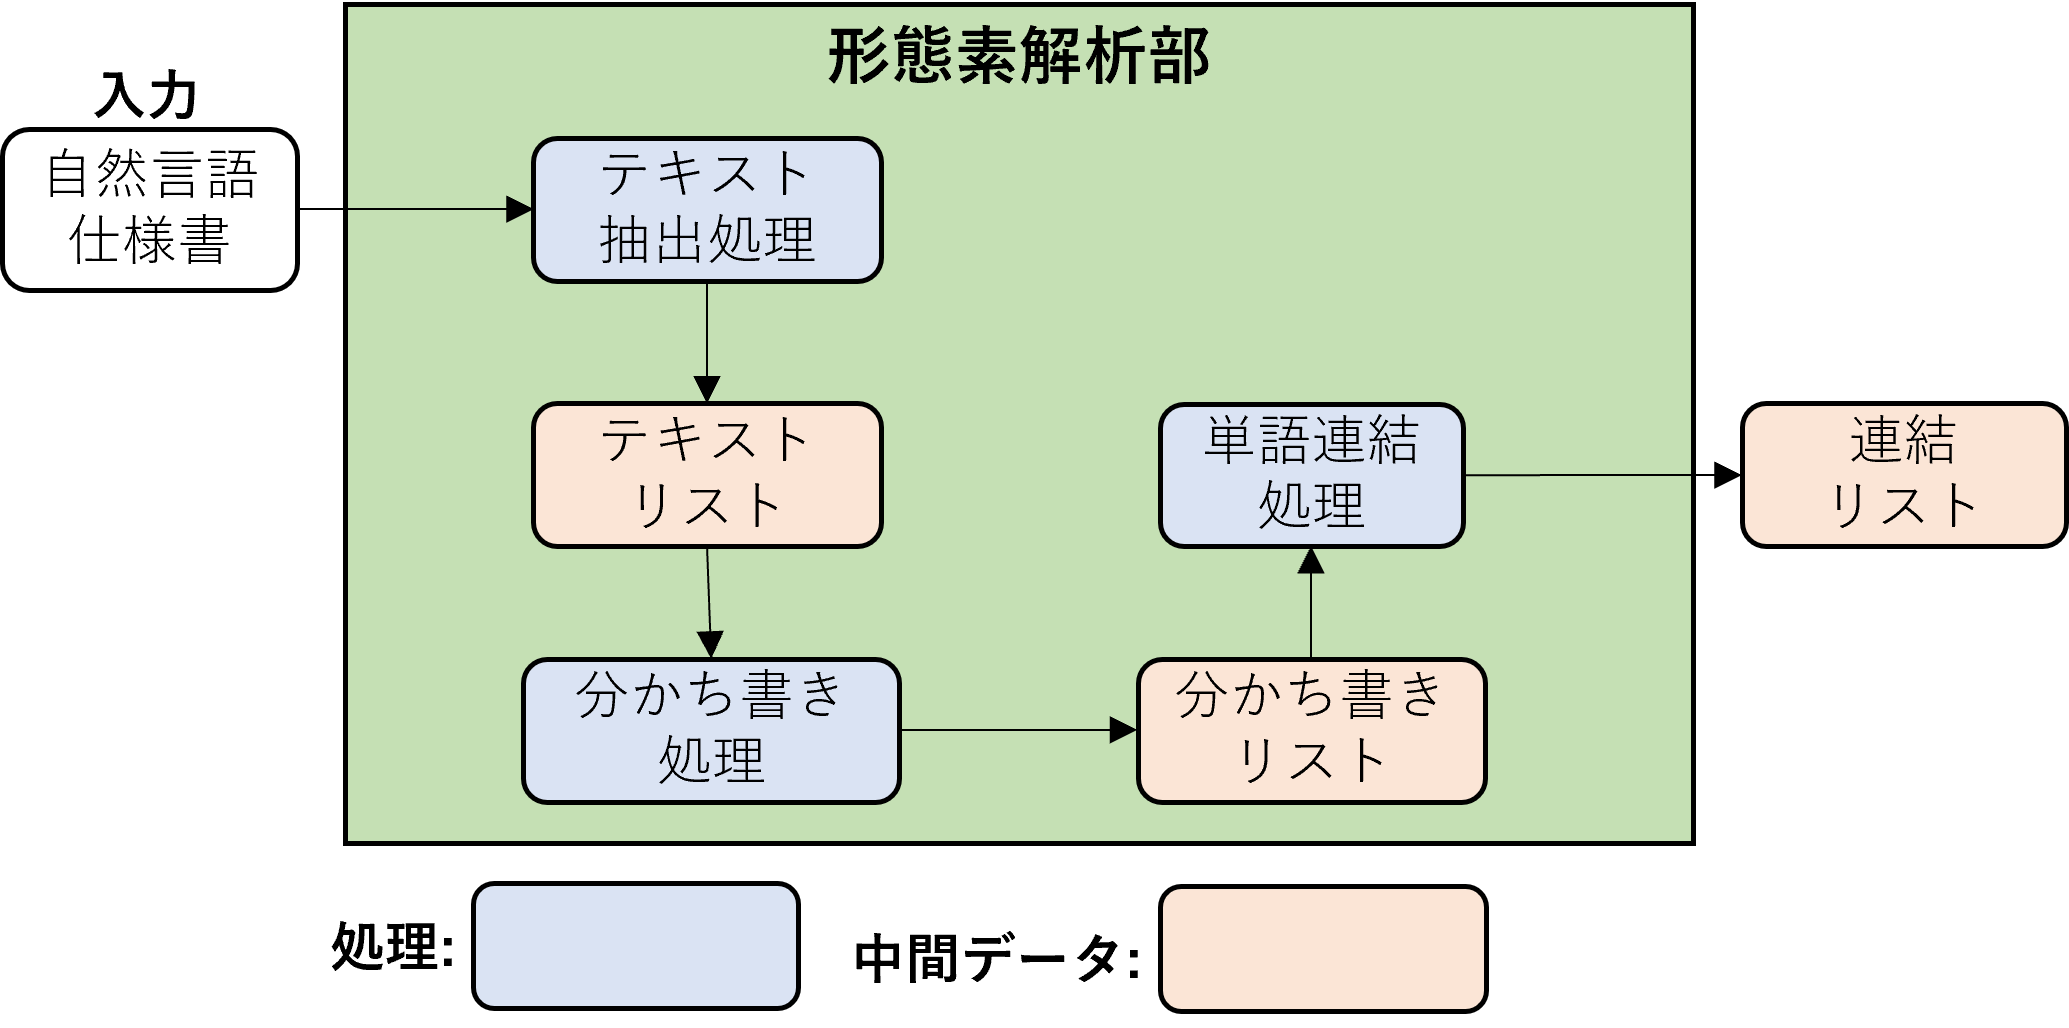
\includegraphics[width=1.0\columnwidth]{image/exis_mor_structure.png}
        \caption{既存手法における形態素解析部の構造}
        \label{fig:exis_mor_structure}
    \end{center}
\end{figure}

\begin{figure}[tp]
    \begin{center}
        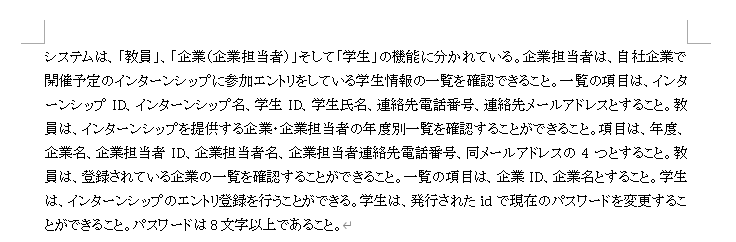
\includegraphics[width=1.0\columnwidth]{image/exis_spec_example.png}
        \caption{入力とする自然言語仕様書の例}
        \label{fig:exis_spec_example}
    \end{center}
\end{figure}

\begin{figure}[tp]
    \begin{center}
        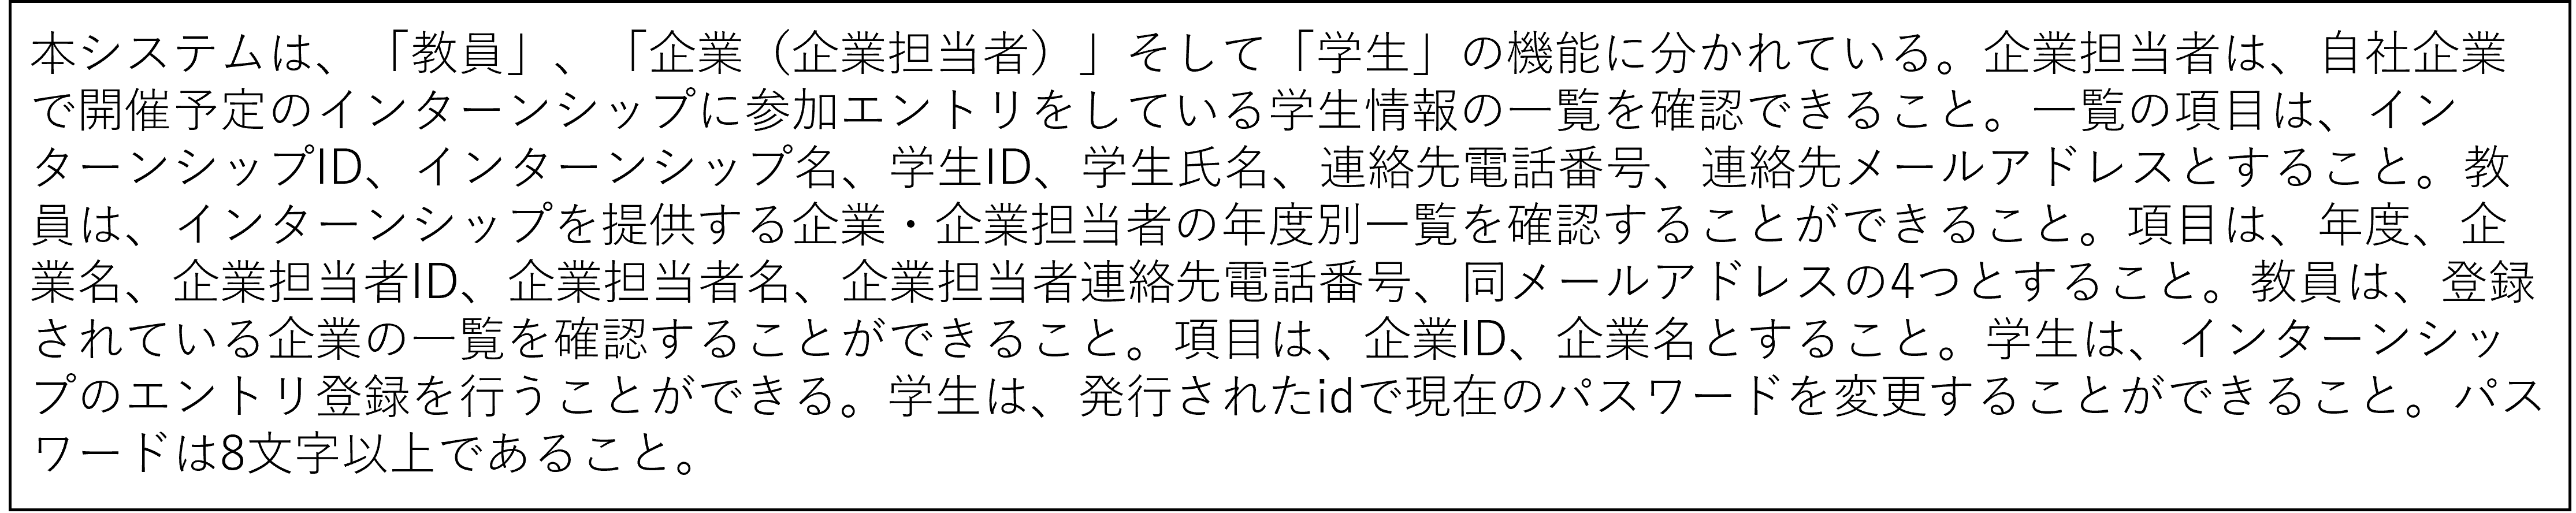
\includegraphics[width=1.0\columnwidth]{image/exis_text_list.png}
        \caption{既存手法のテキスト抽出処理が生成するテキストリスト}
        \label{fig:exis_test_list}
    \end{center}
\end{figure}

\begin{figure}[tp]
    \begin{center}
        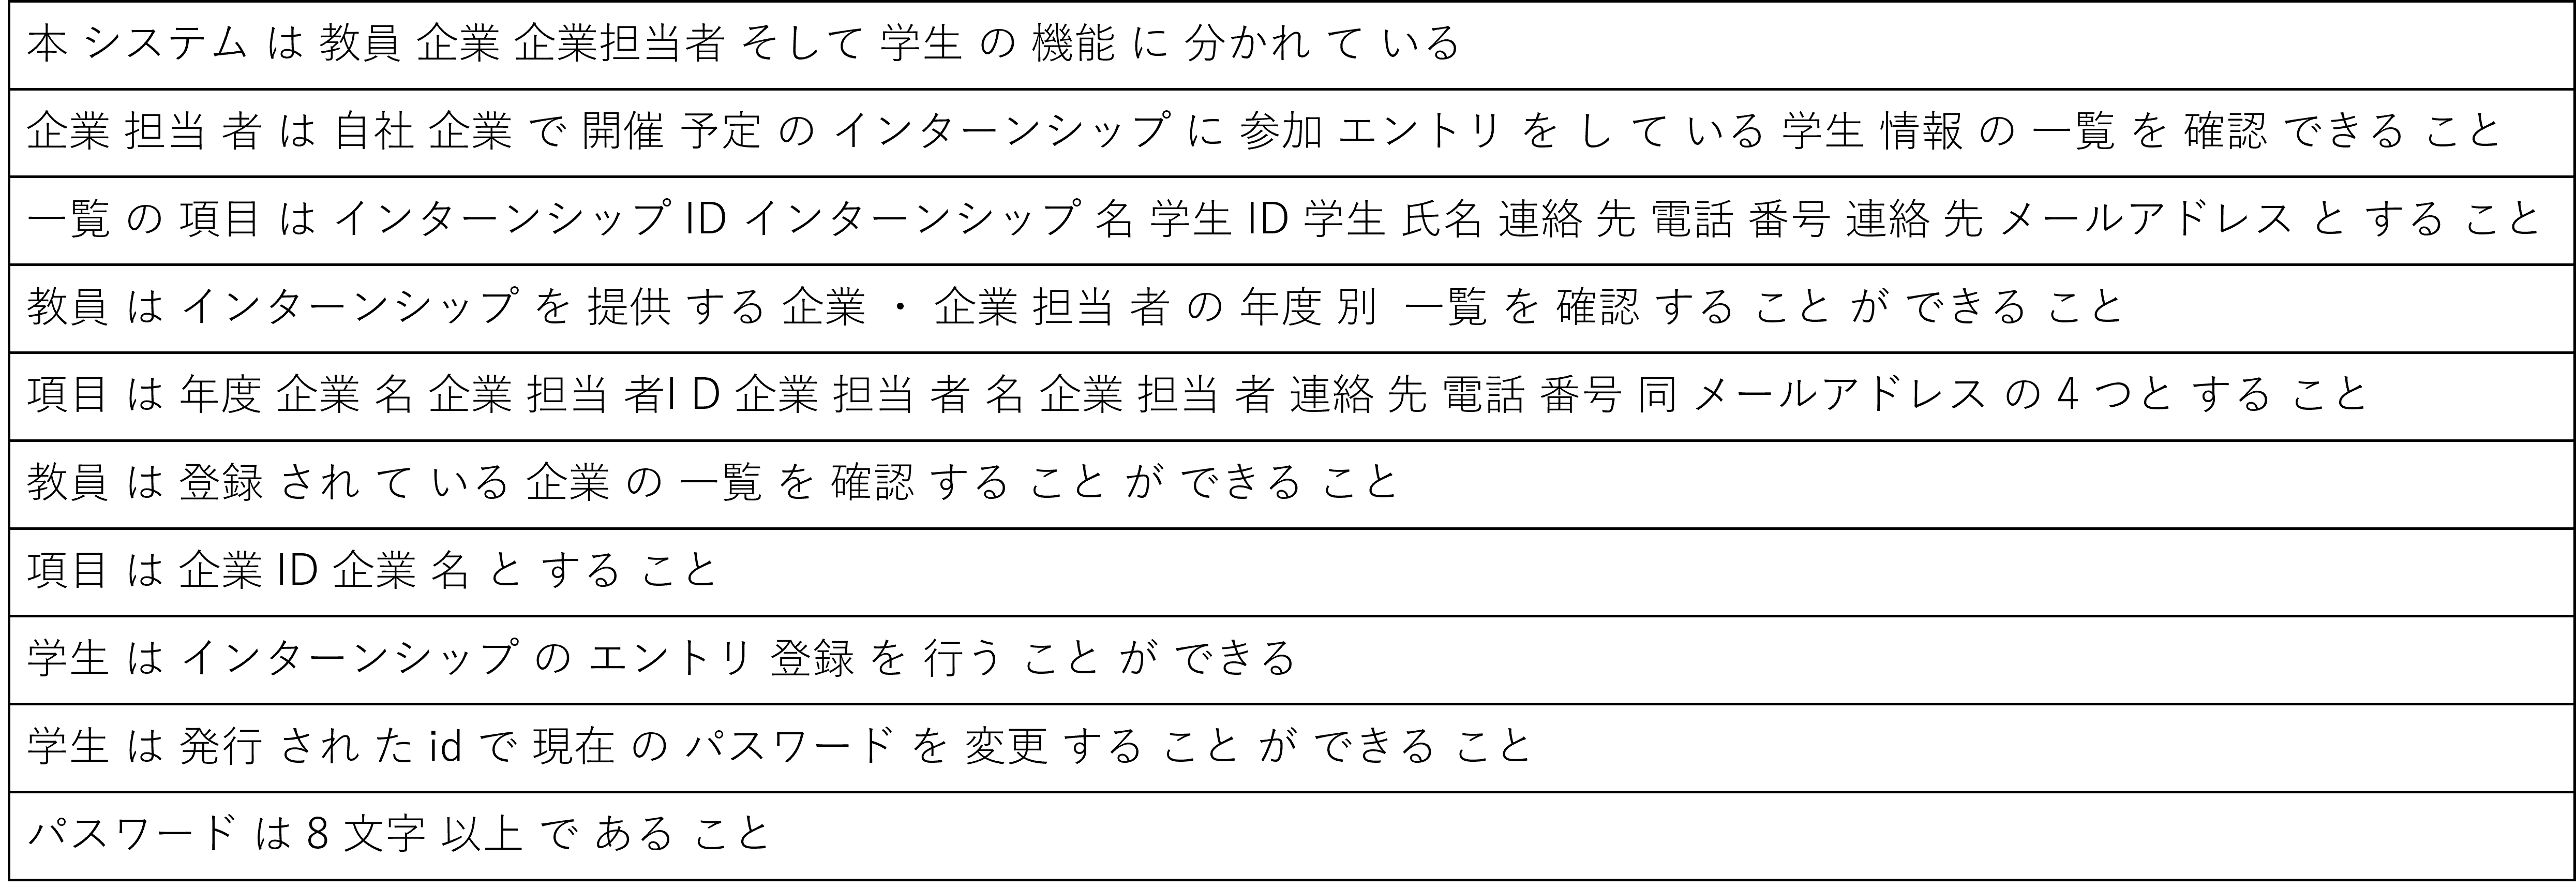
\includegraphics[width=1.0\columnwidth]{image/exis_wakati_list.png}
        \caption{既存手法の分かち書き処理が生成する分かち書きリスト}
        \label{fig:exis_wakati_list}
    \end{center}
\end{figure}

\begin{figure}[tp]
    \begin{center}
        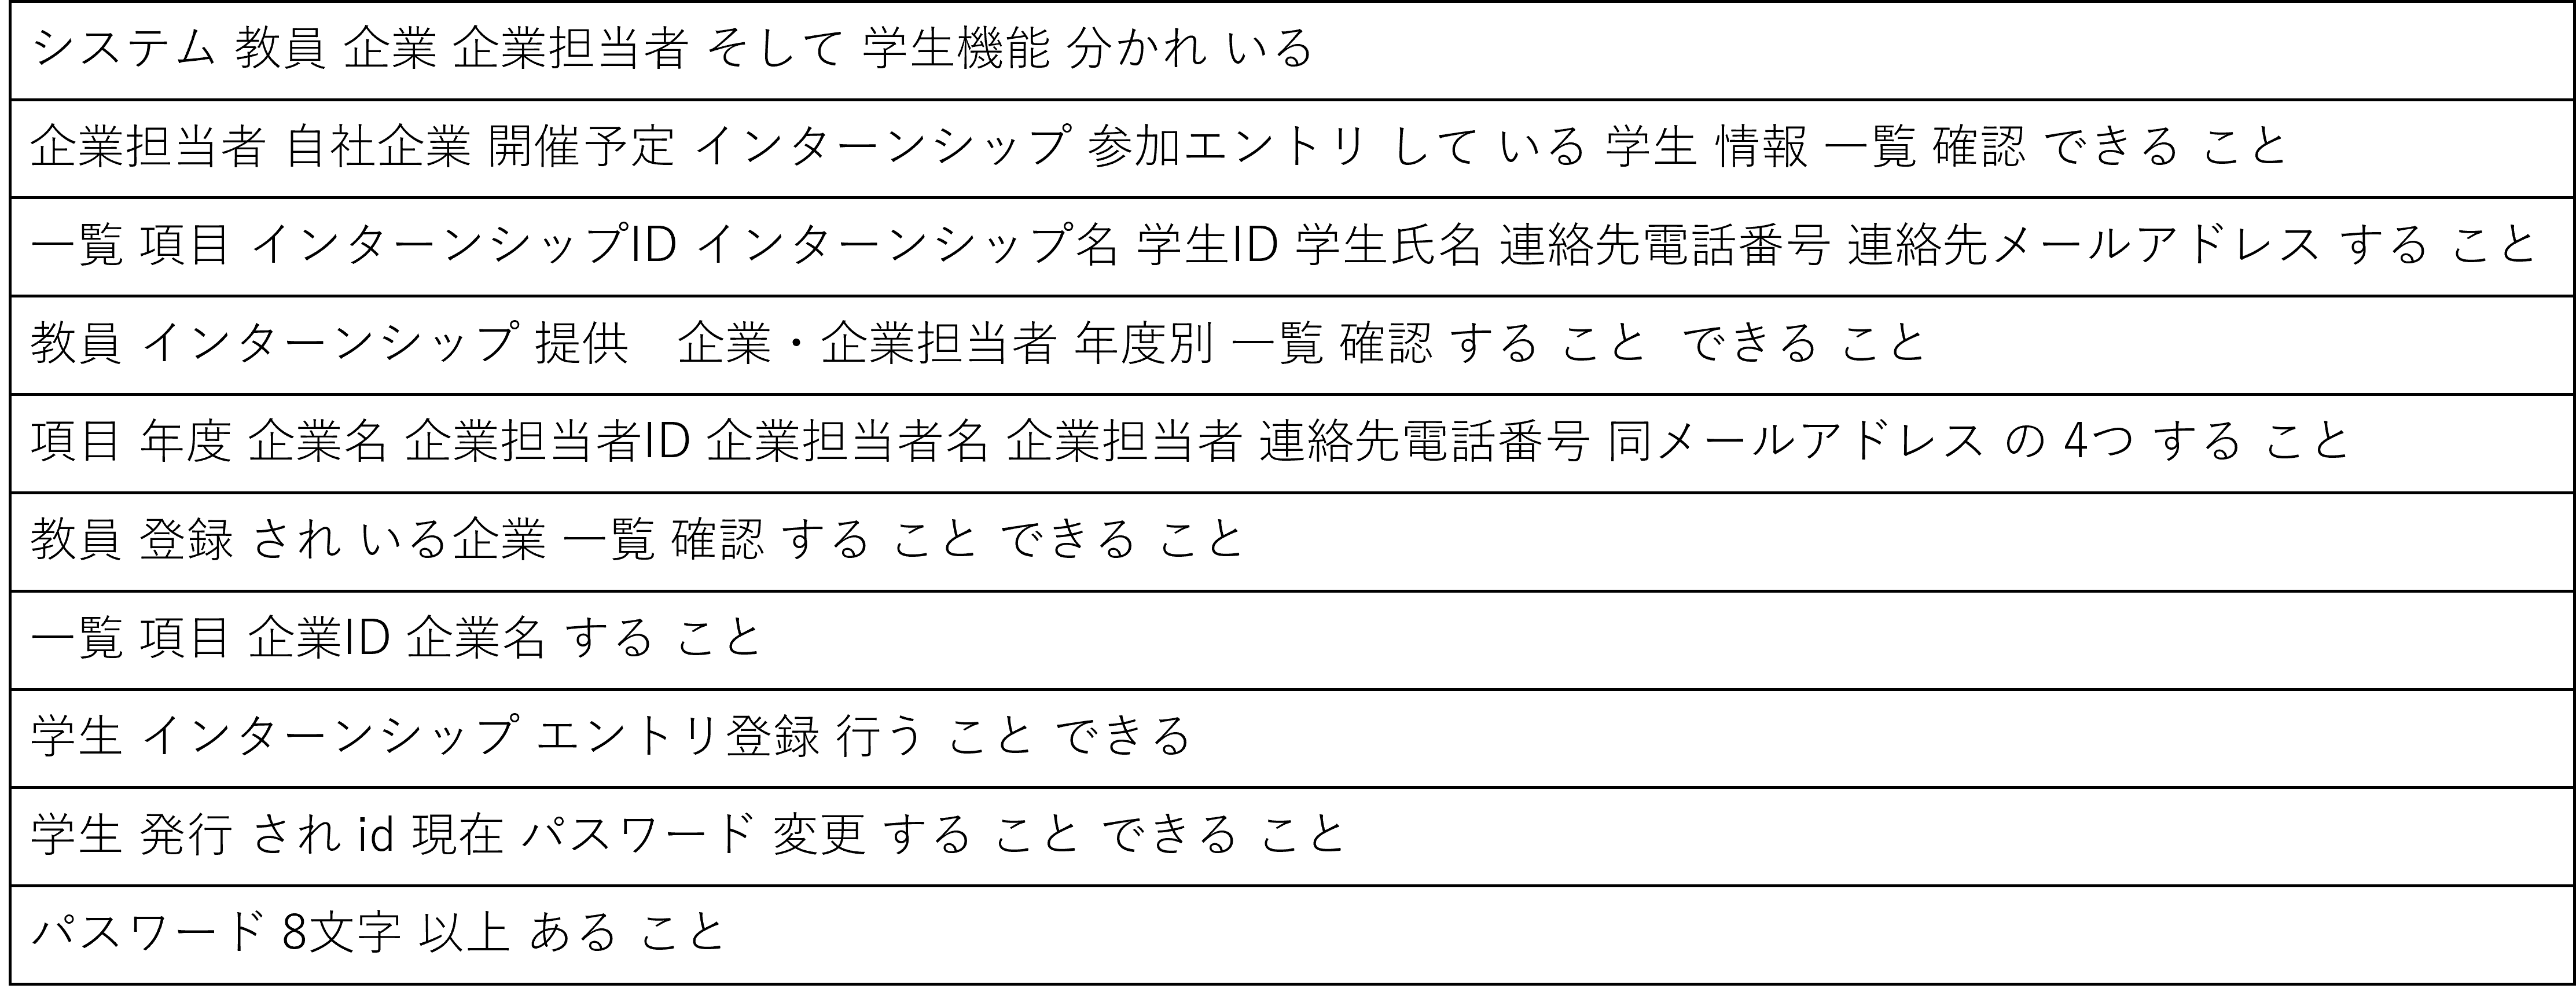
\includegraphics[width=1.0\columnwidth]{image/exis_connect_list.png}
        \caption{既存手法の形態素解析部が生成する連結リスト}
        \label{fig:exis_connect_list}
    \end{center}
\end{figure}

\section{変換部}
\label{sec:exis_transfer}
既存手法における変換部は、図\ref{fig:exis_connect_list}に示す連結リストを入力として、単語リストを生成する。
既存手法における変換部の構造を、図\ref{fig:exis_transfer_structure}に示す。
既存手法における変換部の処理の流れを、以下に示す。

\begin{enumerate}
    \item TF-IDF値生成処理において、図\ref{fig:exis_connect_list}に示す連結リストを入力とし、連結リスト内の単語に対し\ref{}で述べたTF-IDF値を計算する。さらに、連結リスト内の単語を全て格納した単語配列と、単語とTF-IDF値のセットを格納した列数2の一時ファイルを生成する。
    \label{tf_list}
    \item 出現回数生成処理において、\ref{tf_list}で生成した単語配列と列数2の一時ファイルを入力とし、単語配列の各単語の出現回数を計算する。さらに、列数2の一時ファイルに各単語の出現回数を追加することによって列数3の一時ファイルを生成する。
    \label{appear_list}
    \item 優先値生成処理において、\ref{appear_list}で生成した列数3の一時ファイルを入力とし、各単語の文字数とその文字の種類によって重みづけをした値(優先値)を計算する。さらに、列数3の一時ファイルに各単語の優先値を追加することによって列数4の一時ファイルを生成する。文字の種類によって重みづけをした値を表\ref{}に、優先値の計算式を式\ref{}に示す。
    \label{prior_list}
    \item 連結回数生成処理において、図\ref{fig:exis_connect_list}に示す連結リストと\ref{prior_list}で生成した列数4の一時ファイルを入力とし、各単語が他の単語に連結している回数を計算する。さらに、列数4の一時ファイルに各単語の連結回数を追加することによって単語リストを生成する。
    \label{exis_word_list}
    \item 数値抽出処理において、図\ref{fig:exis_connect_list}に示す連結リストと\ref{exis_word_list}で生成した単語リストを入力とし、各単語が同じ文中にその単語の数を表す数値があるかを探索する。さらに、単語、数値、TF-IDF値のセットを格納した数値リストを生成する。
\end{enumerate}

図\ref{fig:exis_connect_list}に示す連結リストを入力として、既存手法の変換部が生成する単語リストの一部を図\ref{fig:exis_connect_list}に、数値リストを図\ref{fig:exis_suti_list}示す。

\begin{figure}[tp]
    \begin{center}
        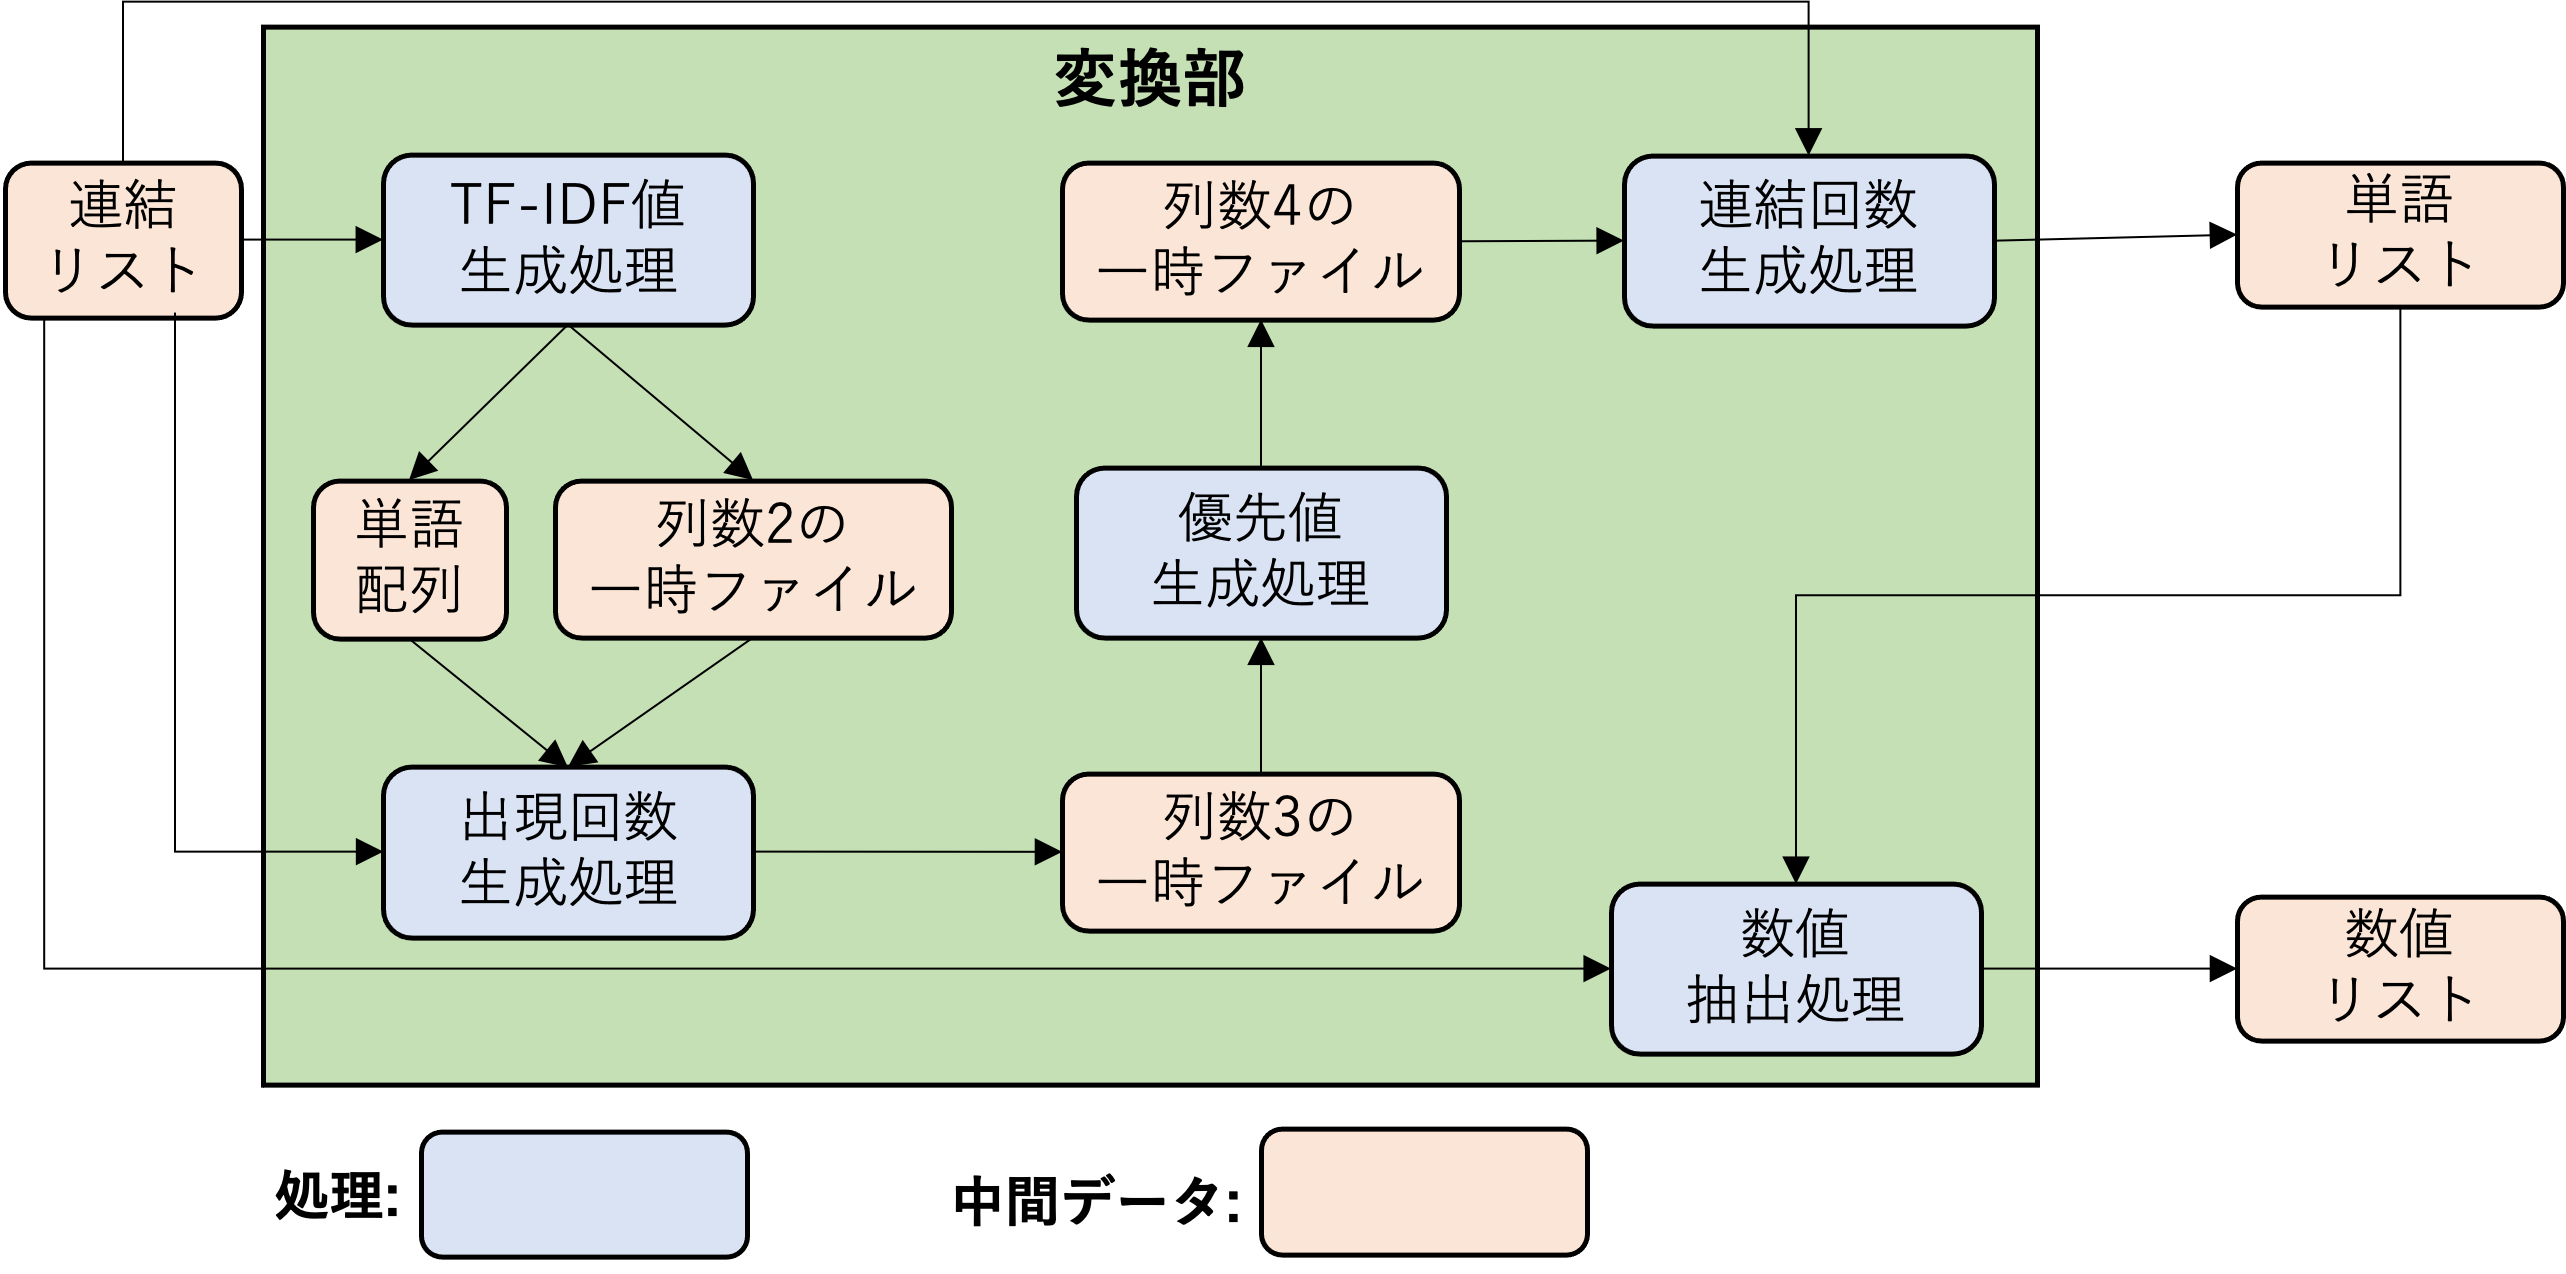
\includegraphics[width=1.0\columnwidth]{image/exis_transfer_structure.png}
        \caption{既存手法における変換部の構造}
        \label{fig:exis_transfer_structure}
    \end{center}
\end{figure}

\begin{figure}[tp]
    \begin{center}
        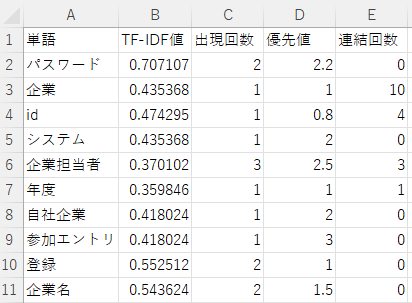
\includegraphics[width=300]{image/exis_word_list.png}
        \caption{既存手法の変換部が生成する単語リストの一部}
        \label{fig:exis_word_list}
    \end{center}
\end{figure}

\begin{figure}[tp]
    \begin{center}
        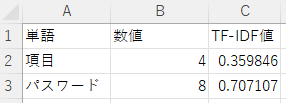
\includegraphics[width=180]{image/exis_suti_list.png}
        \caption{既存手法の変換部が生成する数値リスト}
        \label{fig:exis_suti_list}
    \end{center}
\end{figure}

\section{機械学習部}
\label{sec:exis_machine}
既存手法における機械学習部は、2つの役割を持つ。1つは、前処理として、教師データを入力とし、学習済みモデルを出力する。
もう一つは、単語リストと学習済みモデルを入力とし、判定リストを出力する。
既存手法における機械学習部の構造を、図\ref{fig:exis_machine_structure}に、既存手法の機械学習部が入力とする教師データの一部を、図\ref{fig:exis_teach}に示す。
また、学習済みモデルについては、「インターンシップ評定書・オンライン提出システム」によって生成した学習済みモデルを使用する。
「インターンシップ評定書・オンライン提出システム」は、宮崎大学工学部情報システム工学科の演習科目「プログラミング演習5」の課題として使用された自然言語仕様書である。
付録A.に、「インターンシップ評定書・オンライン提出システム」の自然言語仕様書を示す。
既存手法の機械学習部が入力する教師データは、図\ref{fig:exis_word_list}に示す単語リストの単語の次の列に判定結果の列を挿入したものである。判定結果は、0または1の値を人手により与える。
0は単語がVDM++仕様書に必要でないことを表し、1は単語がVDM++仕様書に必要であることを表す。

表\ref{table:exis_data_set}に既存手法における教師あり学習のデータセット数を示す。

\begin{table}[t]
    \begin{center}
      \caption{既存手法における教師データのデータセット数}
      \label{table:exis_data_set}
      \begin{tabular}{c|c}
        データ総数 & 157\\
        \hline
        \hline
        VDM++仕様書に必要であるデータ    & 71\\ \hline
        VDM++仕様書に必要でないデータ & 86\\ \hline
      \end{tabular}
    \end{center}
  \end{table}

既存手法における機械学習部の処理の流れを、以下に示す。

\begin{enumerate}
    \item 学習済みモデル生成処理において、図\ref{fig:exis_teach}に示す教師データを入力とし、\ref{}節で述べた二項ロジスティック回帰分析を用いて学習済みモデルを生成する。
    \label{exis_teach_model}
    \item 判定リスト生成処理において、\ref{exis_teach_model}で生成した学習済みモデルと図\ref{exis_word_list}に示す単語リストを入力とし、単語リスト内の単語がVDM++仕様書に必要である確率を計算する。さらに、確率が0.5未満である単語に0の判定結果を、確率が0.5以上の単語に1の判定結果を与える。最後に、単語リストに単語の判定結果と確率を追加することによって判定リストを生成する。
\end{enumerate}

図\ref{fig:exis_teach}に示す教師データを基に生成した学習済みモデルと、図\ref{fig:exis_word_list}に示す単語リストを入力として、既存手法の機械学習部が生成する判定リストの一部を図\ref{fig:exis_judge_list}に示す。

\begin{figure}[tp]
    \begin{center}
        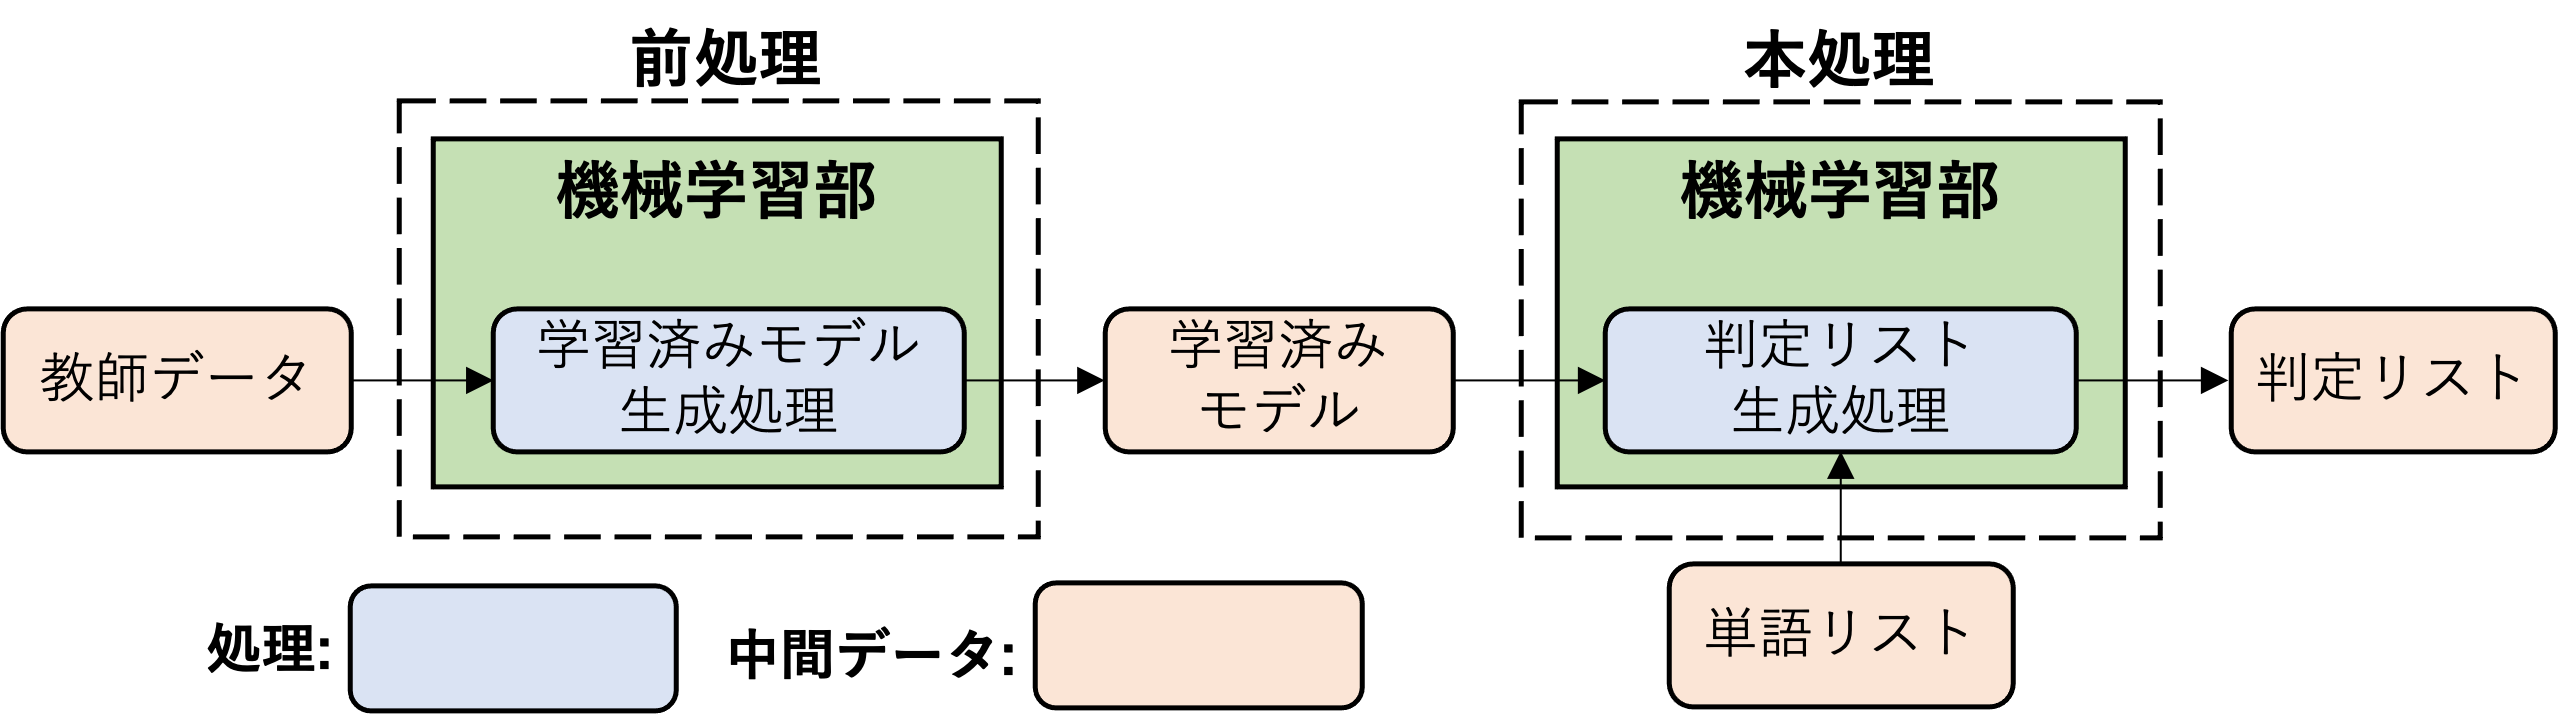
\includegraphics[width=1.0\columnwidth]{image/exis_machine_structure.png}
        \caption{既存手法における機械学習部の構造}
        \label{fig:exis_machine_structure}
    \end{center}
\end{figure}

\begin{figure}[tp]
    \begin{center}
        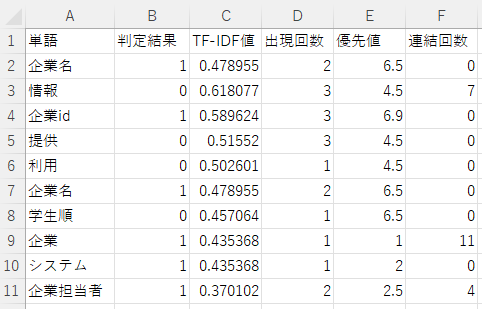
\includegraphics[width=300]{image/exis_teach.png}
        \caption{既存手法の機械学習部が入力とする教師データの一部}
        \label{fig:exis_teach}
    \end{center}
\end{figure}

\begin{figure}[tp]
    \begin{center}
        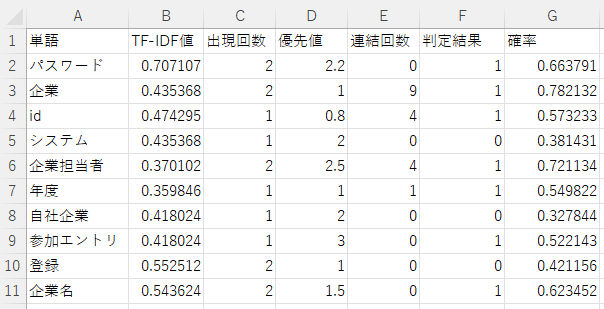
\includegraphics[width=300]{image/exis_judge_list.png}
        \caption{既存手法の機械学習部が生成する判定リストの一部}
        \label{fig:exis_judge_list}
    \end{center}
\end{figure}

\section{VDM++仕様書生成部}
既存手法におけるVDM++仕様書生成部は、図\ref{fig:exis_judge_list}に示す判定リストを入力として、VDM++仕様書を生成する。
既存手法におけるVDM++仕様書生成部の構造を、図\ref{fig:exis_generator_structure}に示す。
既存手法におけるVDM++仕様書生成部の処理の流れを、以下に示す。

\begin{enumerate}
    \item 型・定数定義生成処理において、図\ref{fig:exis_suti_list}に示す数値リストと、図\ref{fig:exis_judge_list}に示す判定リストを入力とし、識別子を挿入するための一時的なID「INDEX」と単語のセット、または「INDEX」、単語、数値のセットを格納した型・定数定義リストを生成する。図\ref{fig:exis_suti_list}と図\ref{fig:exis_judge_list}を入力として、既存手法の型・定数定義生成処理が生成する型・定数定義リストを、図\ref{fig:exis_katateisu_list}に示す。
    \label{katateisu}
    \item 識別子挿入処理において、\ref{katateisu}で生成した型・定数定義リスト内の一時的なID「INDEX」に、「types」または「values」を識別子として挿入する。さらに、識別子と単語のセット、または識別子、単語、数値のセットを格納した型・定数定義識別子リストを生成する。図\ref{fig:exis_katateisu_list}に示す型・定数定義リストを入力として、既存手法の識別子挿入処理が生成する型・定数定義識別子リストを、図\ref{fig:exis_katateisu_id_list}に示す。
    \label{sikibetu}
    \item VDM++仕様書生成部において、表\ref{table:vdm_syntax}の構文に従って、\ref{sikibetu}で生成した型・定数定義識別子リスト内の単語をVDM++仕様書の構文の「名前」に、数値をVDM++仕様書の構文の「値」に挿入する。さらに、構文に沿って単語と数値を挿入した後の文字列を、ファイルに記述することによってVDM++仕様書を生成する。図\ref{fig:exis_katateisu_id_list}に示す型・定数定義識別子リストを入力として、既存手法のVDM++仕様書生成処理が生成するVDM++仕様書を、図\ref{fig:exis_vdm}に示す。
\end{enumerate}

\begin{figure}[tp]
    \begin{center}
        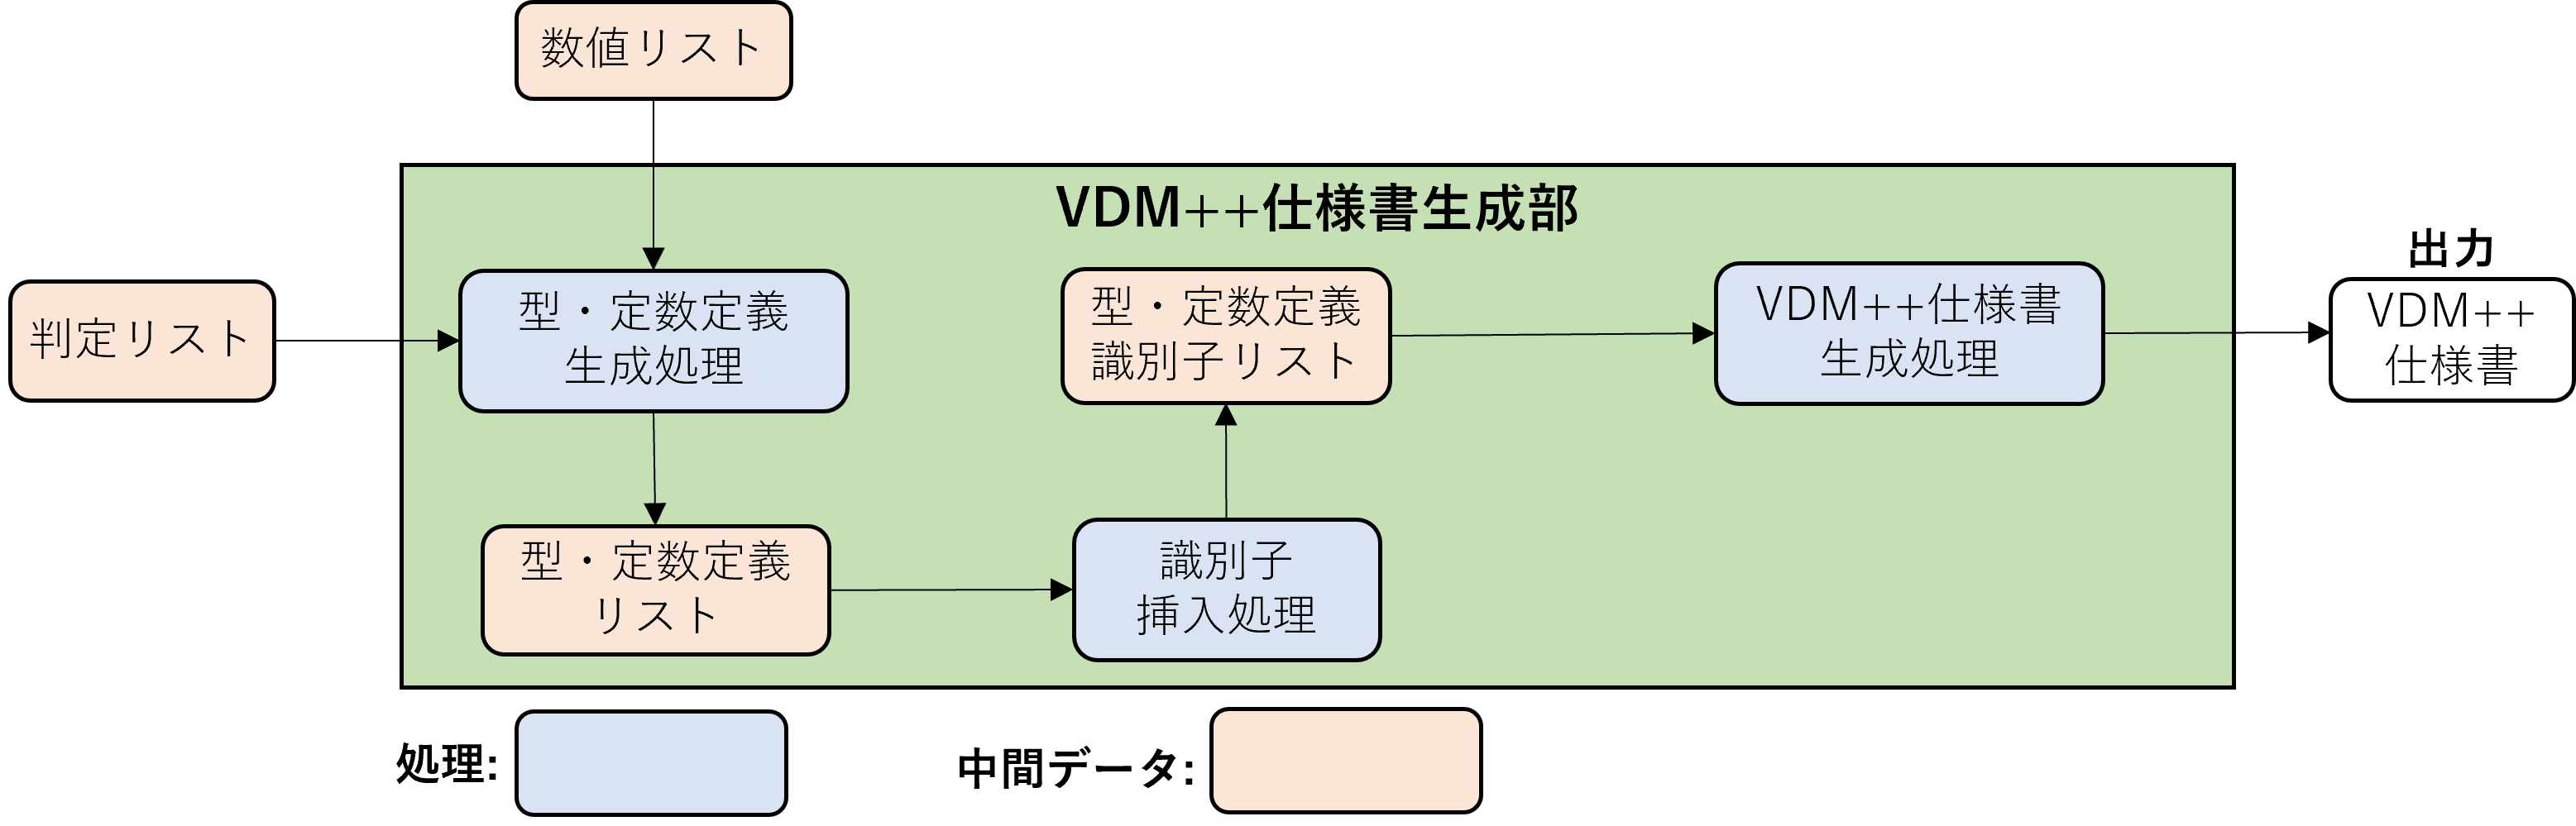
\includegraphics[width=1.0\columnwidth]{image/exis_generator_structure.png}
        \caption{既存手法におけるVDM++仕様書生成部の構造}
        \label{fig:exis_generator_structure}
    \end{center}
\end{figure}

\begin{figure}[tp]
    \begin{center}
        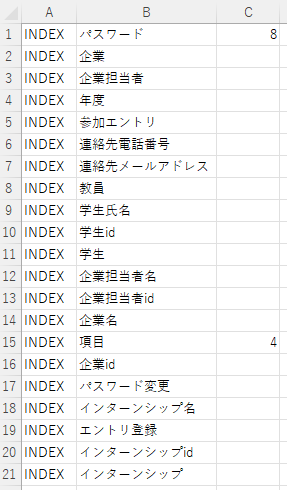
\includegraphics[width=300]{image/exis_katateisu_list.png}
        \caption{既存手法の型・定数定義生成処理が生成する型・定数定義リスト}
        \label{fig:exis_katateisu_list}
    \end{center}
\end{figure}

\begin{figure}[tp]
    \begin{center}
        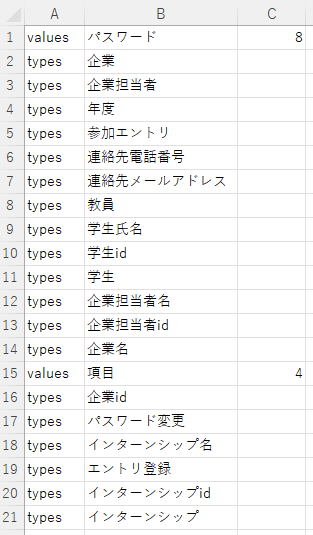
\includegraphics[width=300]{image/exis_katateisu_id_list.PNG}
        \caption{既存手法の識別子挿入処理が生成する型・定数定義識別子リスト}
        \label{fig:exis_katateisu_id_list}
    \end{center}
\end{figure}


\begin{figure}[tp]
    \begin{center}
        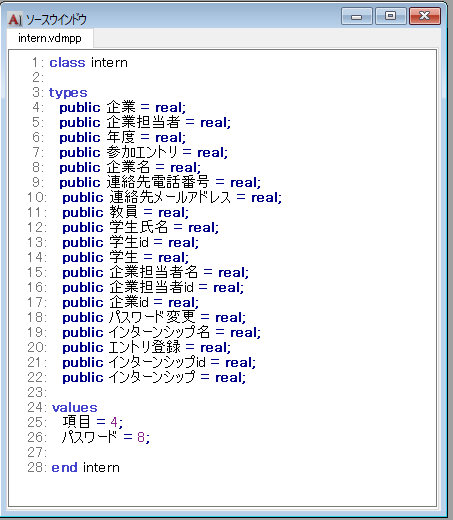
\includegraphics[width=300]{image/exis_vdm.png}
        \caption{既存手法のVDM++仕様書生成処理が生成するVDM++仕様書}
        \label{fig:exis_vdm}
    \end{center}
\end{figure}

\section{既存手法の問題点}
\label{sec:problemm}
既存手法は、上記の4つの処理部によって、自然言語仕様書内の単語の内、VDM++仕様書に必要な単語を抽出し、VDM++仕様書を自動生成することができる。
しかし、既存手法は、自然言語仕様書から抽出した単語を、VDM++仕様書に必要である単語と必要でない単語に分類し、型定義と定数定義に対応したVDM++仕様書を出力できるが、
クラスやその他のブロック定義に対応したVDM++仕様書を出力することができない。そのため、既存手法は、対応しているVDM++の構文が少なく、有用性が低い。
本論文では、既存手法の有用性の向上を目的として、VDM++仕様書における以下の3つの構文を生成する手法を提案する。
さらに、提案手法を既存手法に適用し、機械学習を活用したVDM++仕様書自動生成ツールVGMLを開発する。

\begin{itemize}
    \item クラス
    \item インスタンス変数
    \item 操作定義
\end{itemize}